\section{Previous Work}

\subsection{Compositional Pattern Producing Networks}
\label{sec:cppn}
Compositional Pattern Producing Networks(CPPN) are a type of Artificial Neural Networks(ANN) introduced by Kenneth Stanley\cite{Stanley2007}.
CPPNs use function composition in an effort to obtain repetition, symmetry, and regularities in the produced phenomes.
An example of how functions are combined to form a CPPN can be seen on figure~\ref{fig:cppn}.
\begin{figure}[ht]
\centering
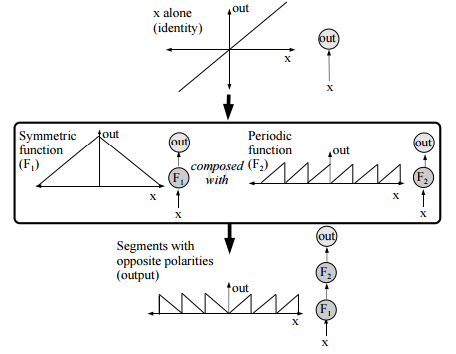
\includegraphics[scale=.5]{cppn}
\caption{An example CPPN as shown in \cite{Stanley2007}}
\label{fig:cppn}
\end{figure}
%Stanley presented some experiments which used CPPNs to evolve two-dimensional images.
%The input to these networks were the x- and y-coordinates of the images, and the single output produced by the CPPN was used to colour the pixel at the given coordinate.

\subsection{Computer evolved tables}
\todo[inline]{Change this title?}
Evolutionary Algorithms have been used to develop similar solutions before. Examples of previous  applications are tables[See~figure~\ref{fig:hornby_tables}] where the optimisation parameters were height of the support structure, stability of the structure, and maximization of surface area.
\begin{figure}[ht]
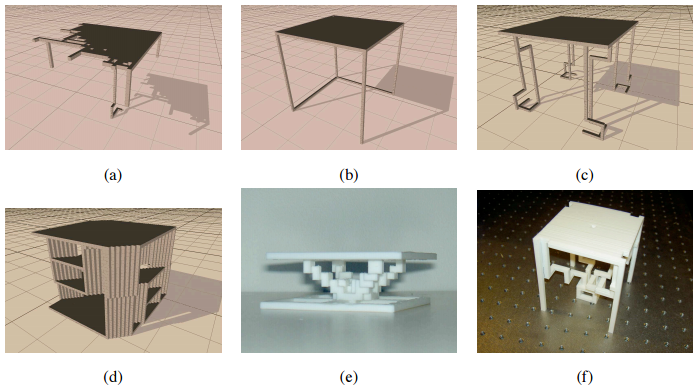
\includegraphics[scale=.6]{content/img/tables}
\caption{Image of Hornby tables\cite{paper:ev4}}
\label{fig:hornby_tables}
\end{figure}

While the evolution of tables has some similarities to seating they are inherently
different in the sense that maximized surface area might not be ideal for a
chair.
Neither would very high legs be optimal, since the physical attributes of humans
usually constrain us to some specific height range which is optimal for the
average persons seating comfort.

\subsection{Evolving 3D objects with CPPNs}
In their paper from 2011 Klune and Lipson describe how they use CPPNs to evolve 3-dimensional objects\cite{Clune:2011:EOG:2078245.2078246}.
They describe how they encode the 3D objects with CPPNs by feeding the CPPN with three inputs, one each for the x-, y-, and z- coordinates of a 3D voxel space.
The single output of the CPPN for the given coordinates is checked against a threshold, and if it is above the threshold the voxel in those coordinates is considered full, otherwise it is considered empty\cite[p.~5]{Clune:2011:EOG:2078245.2078246}.

